% Preamble
\documentclass[a4paper, 12pt]{article}
\usepackage[margin=1in]{geometry} % Set margin
\usepackage{pdfpages} % Insert pdf pages
\usepackage{amssymb,amsmath,amsthm, amsfonts} % Math libraries

% Custom commands
\newcommand{\sub}[1]{\subsection{\underline{#1}}}
\newcommand{\subsub}[1]{\subsubsection{\underline{#1}}}
\newcommand{\R}{\ensuremath{\mathbb{R}}}
\newcommand{\F}{\ensuremath{\mathbb{F}}}
\newcommand{\N}{\ensuremath{\mathbb{N}}}
\newcommand{\Onef}{\ensuremath{1_{\F}}}
\newcommand{\Zerof}{\ensuremath{0_{\F}}}
\newcommand{\eqbcuz}[1]{\text{~$\stackrel{(#1)}{=}$~}}
\newcommand{\eq}[1]{\begin{align*}#1\end{align*}}
\newcommand{\eqn}[1]{\begin{align}#1\end{align}}
\renewcommand{\qed}{\hfill\(\qedsymbol\)}
\newtheorem{lemma}{Lemma}

% Begin Document %
\begin{document}

% Title Page
\begin{titlepage}
    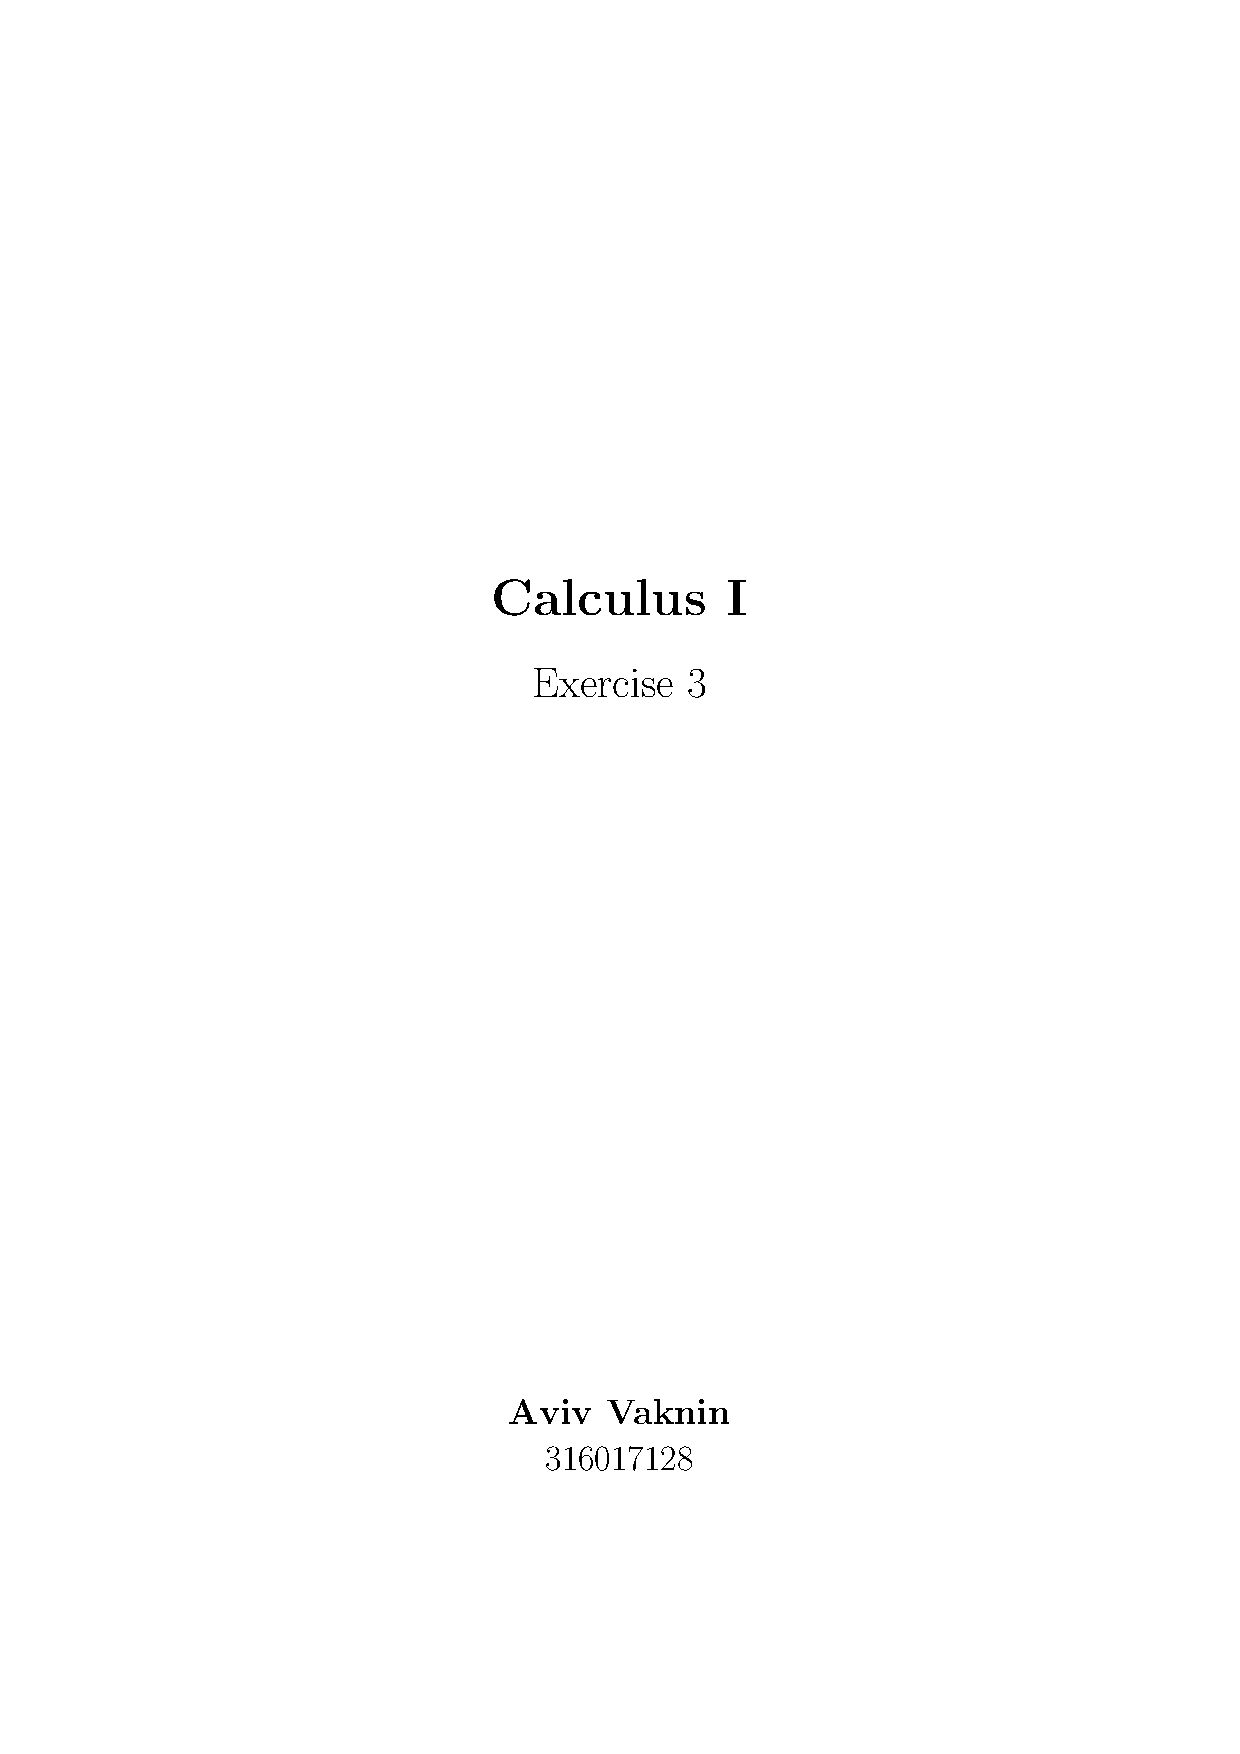
\includepdf{title.pdf}
\end{titlepage}

%1
\section{
$A\subseteq\F$, prove $m\in\F$ is the infimum of A \underline{\textit{if and only if}}:}
\begin{enumerate}
    \item m is the lower bound of $A$
    \item $(\forall\epsilon>0)~(\exists{a}\in{A})~(a<m+\epsilon)$
\end{enumerate}
\sub{$\implies$:}
We'll start with assuming $m\in\F$ is the infimum of $A$.\\
By definition, the infimum is a lower bound \textbf{(1)}.\\
Therefore: \eq{\forall{a}\in{A}~~a\geq{m}}
and, suppose $m'$ is another lower bound for $A$: \eq{m\geq{m'}}
First, by definition, an infimum is a lower bound.\\
Regarding the second item, let's suppose by contradiction:
\eq{\exists\epsilon>0~~\forall{a}\in{A}~~a\geq{m+\epsilon}\\m+\epsilon>m}
Therefore, we can see that $\underline{m+\epsilon}$ is a lower bound for $A$, bigger than the infimum.\\
We've reached a contradiction, as we've assumed $m$ is the infimum of $A$ \textbf{(2)}.
\sub{$\impliedby$:}
Let's suppose that $m$ is not the infimum.\\
Therefore, exists another lower-bound - $m'$ so that $m'>m$.\\
Let $\epsilon>0$: \eq{\epsilon=m'-m\\m'=\epsilon+m}
Therefore: \eq{\forall\epsilon>0~~\exists{a}\in{A}~~a\geq\epsilon+m}
Which is in contradiction with our initial assumption: \eq{(\forall\epsilon>0)~(\exists{a}\in{A})~(a<m+\epsilon)}
\qed\pagebreak

%2
\section{\eq{A\subseteq\F\\s\in\F}}
\sub{Prove $s=\max(A) \iff (s=\sup(A)) \land (s\in{A})$}
\subsub{$\implies$:}
Let's start by supposing $s=\max(A)$.\\
By definition, the maximum is always part of the set, therefore \textbf{(1)}: \eq{s\in{A}}
Let's show that $\max(A)=\sup(A)$:\\
We know from definition, that \textit{s} is an upper-bound of $A$.\\
Let's take any arbitrary $\epsilon>0$, therefore because $s\in{A}$:
\eq{s>s-\epsilon}
Therefore, by the definition of the supremum(proposition 5.7 in class), $s$ is $A$'s supremum.\textbf{(2)}
\subsub{$\impliedby$:}
Let's suppose that $s=\sup(A)$ and $s\in{A}$.\\
According to the definition of the maximum, if $s$ is the maximum of $A$, it must be:
\begin{enumerate}
    \item a member of $A$
    \item a supremum of $A$
\end{enumerate}
Both are given.
\qed
\sub{Prove that if $A$ has a maximum, there's only one.}
By definition, if a set has a maximum, it fulfills the following properties:
\begin{enumerate}
    \item it is a member of the set
    \item it is a supremum of the set
\end{enumerate}
Suppose $m$ is the maximum of $A$.\\
By definition, it must be part of $A$, satisfying \textbf{(1)}.
Because of \textbf{(2)}, it must be a supremum.
\subsub{n's smaller than m}
According to the definition of the upper-bound: \eq{\forall{\epsilon}>0~~\exists{a}\in{A}~~a>m-\epsilon}
Therefore, $m-\epsilon$ is smaller than $m$, and is not an upper-bound, therefore not a maxmium.
\subsub{n's bigger than m}
Likewise, $m+\epsilon$ is bigger than $m$, and is by definition an upper-bound.\\
However, we've stated that m is the upper-bound of $A$, and according to the upper-bound definition,\\
Every number that is bigger than the upper-bound of a set, is not a member of the set.\\
Therfore, we've shown that there can only exist a single maximum, if any.
\qed

%3
\section{$\varnothing\neq A,B\subseteq\F$\\Prove or disprove:}
\sub{}
Let $A=\R$, and $B=\N$.\\
Therefore, we can see that \textit{A} is not lower-bounded, while \textit{B} is lower-bounded by 1.
Disproved.\qed
\sub{}
If the claim is incorrect, then \textit{B} mustn't have an upper-bound.\\
Since \textit{B} is a subset of \textit{A}, \textit{B} must be bounded from above as well, that is due to the definition of an upper bound.\\
In formal notation, as $B\subseteq{A}$:
\eq{(\forall{b}\in{B})~(\exists{a}\in{A})~(a\geq{b})}
However, since \textit{A} is bounded from above: \eq{(\forall{a}\in{A})~(\exists{m})~(m\geq{a})}
Therefore, due to transitivity: \eq{m\geq{b}}
\qed\pagebreak

%4
\section{$\varnothing\neq A,B\subseteq\F~~\exists\sup(A),\exists\sup(B)$\\Prove or disprove:}
\sub{$B\subseteq{A} \implies \sup(B)\leq\sup(A)$}
Let $m=\sup(A)=\max(A)$.\\
Therefore, according to the definition of the \textit{supremum}:
\eq{\forall{a}\in{A}~m\geq{a}}
Now, let's take a look at the maximum of \textit{B}:
\eq{\forall{b}\in{B}~m'\geq{b}}
Since $B\subseteq{A}$, the maximum value of \textit{B} can, at the most be equal to \textit{m}, that is: \eq{m'\leq{m}}
\qed
\sub{$(B\subseteq{A})~\land~(B\neq{A})\implies \sup(B)<\sup(A)$}
Let: \eq{A=\{1,2,3\}\\B=A\backslash\{1\}}
We can clearly see that $(B\subseteq{A})~\land~(B\neq{A})$.\\
However, $\sup(B)=\sup(A)=3$, thus the claim is incorrect.
\qed
\sub{$-A=\{-a~|~a\in{A}\}$}
It is given that \textit{A} necessarily has a supremum.\\
Therefore, \textit{-A} is necessarily bounded from below by that same supremum, as a negative.\\
Let \textit{m} be \textit{A}'s supremum, and \textit{-m} be \textit{-A}'s infimum.\\
According to the definition of the \textit{supremum}:
\eq{\forall{a}\in{A}~m\geq{a}}
We'll multiply by \textit{(-1)}:
\eq{
    -m\leq{-a}
}
Note that this is exactly the definition of the infimum.
Thus, we can conclude that \textit{-A} is bounded from below, $\exists\inf(-A)$ and that $\inf(-A)=-\sup(A)$.
\qed\pagebreak

%5
\section{}
\sub{$A=\{x^2+7x+10~|~x\in\F\}$}
First, we'll pack $x^2+7x+10$ into $(x+5)(x+2)$ and get: \eq{A=\{(x+5)(x+2)~|~x\in\F\}}
\subsub{upper-bound, supremum \& maximum}
Now, it is easier to see that as \textit{x} gets bigger, the equation gets bigger.\\
According to \textit{definition 5.1}, a set is bounded from above only if: \eq{(\exists{M}\in\F)~(\forall{a}\in{A})~(a\leq{M})}
However, there doesn't exist such an M, because for every upper bound that we'll test, the equation can yield a bigger number.\\
Because of that, we can conclude that \textit{A} is \textbf{not} bounded from above, and therefore, there doesn't exist either a supremum nor a maximum.
\subsub{lower-bound, infimum \& minimum}
We can rewrite $x^2+7x+10$:
\eq{
    x^2+7x+10&=x^2+7x+10+2.25-2.25\\
    &=(x+3.5)^2-2.25
}
We know that $(x+3.5)^2\geq{0}$, therefore:
\eq{
    (x+3.5)^2-2.25&\geq{-2.25}\\
    x^2+7x+10&\geq{-2.25}
}
Therefore, the lowest value that can be received from the equation is $-2.25$, i.e.: \eq{inf(A)=-2.25}
since $-2.25$ is a member of \textit{A} - as we can place $x=-3.5$ to get this value - it is the minimum as well, i.e.:
\eq{min(A)=inf(A)=-2.25}
\pagebreak
\sub{$B=\{x\in\F~|~x^2+7x+10>0\}$}
Similiar to set A, we'll pack:
\eq{x^2+7x+10=(x+5)(x+2)}
Therefore: \eq{B=\{x\in\F~|~(x+5)(x+2)>0\}}
Therefore, the only members in \textit{B} are all of the \textit{x}'s that will yield positive numbers.\\
As we've shown for \textit{A}, the members therefore are: \eq{B=\{x\in\F~|~(x<-5)\lor(-2<x)\}}
\subsub{upper-bound, supremum \& maximum}
As \textit{x} can be any \textit{x} that is bigger than -2, we can see that it is not bounded from above.
Therefore, the supremum \& maximum do not exist as well.
\subsub{lower-bound, infimum \& minimum}
Similiarly, the value of \textit{x} can always be lower, which is in contrast to the definition of the lower-bound:
\eq{(\exists{m}\in\F)~(\forall{b}\in{B})~(b\geq{m})}
Let's assume that such an \textit{m} \textbf{does} exist.\\
Let's assume that $b=m$, if we add (-1) to \textit{b}, we'll get a member that is still in the set,
as we can always find a smaller member of \textit{B}.\\
And in more formal notation:
\eq{
    &b=m\in\F\\
    &b-1\in\F\\
    &b-1<m
}
Which contradicts the definition of the lower-bound.\\
Therefore, the lower-bound (and as a result of this the infimum and the minimum) doesn't exist.
\pagebreak

%6
\section{}
\sub{The lower-bound property:}
{\Large{In \R, there exists an infimum for every non-empty set that is bounded from below.}}
\sub{}
\subsub{lower-bound property $\implies$ Completeness of the real numbers}
In order to demonstrate the completeness axiom, we need to show that:
\eq{(\forall{A,B}\subset\F)(\exists{c}\in\F)(\forall{a}\in{A})(\forall{b}\in{B})(a\leq{b})(a\leq{c}\leq{b})}
Let $\varnothing\neq{B}\subset\R$ that is bounded from below.\\
According to the lower-bound property - there exists an infimum $c\in\R$ such that:
\eq{(\forall{b}\in{B})~(c\leq{b})}
Now, let's form a new group that contains only $\inf(B)$: \eq{A=\big\{\inf(B)\big{\}}}
We've shown that there exists an infimum to B, hence \textit{A} must be non-empty.\\
Therefore, we've shown what was needed.
\subsub{lower-bound property $\impliedby$ Completeness of the real numbers}
Using the completeness axiom, we need to show that a non-empty set, B, that is bounded-from-below, has an infimum.\\
According to definition, in order for a set to have an infimum, M, it must fullfill:
\begin{enumerate}
    \item Be a lower bound of B
    \item $(\forall\epsilon>0)(\exists{b}\in{B})(a<M+\epsilon)$
\end{enumerate}
Let $B\subset\R$ some non-empty set that is bounded from below, and \textit{A}: \eq{A=\big\{x\in\R:~\forall{b}\in{B}~x\leq{b}\big{\}}}
Since B is bounded from below, and A consists of all of the numbers that are less than or equal to all numbers in B, we can assume:
\begin{enumerate}
    \item $A\neq{\varnothing}$
    \item According to the completeness axiom, there exists $c\in\R$ such that B is bounded-from-below by c and A is bounded-from-above by c.
\end{enumerate}
That is: \eq{\forall{a}\in{A}~a&\leq{c}\\\forall{b}\in{B}~b&\geq{c}\\b&\geq{a}}
Therefore, we've shown that \textit{c} is the greatest lower-bound of \textit{B}.
\qed

%7
\section{}
Let $\varnothing\neq A,B\subset\R$ such that:
\eqn{(\forall{a}\in{A})(\forall{b}\in{B})(a\leq{b})}
It is given that: \eqn{(\forall\epsilon>0)~\exists({a}\in{A},~{b}\in{B})~(b-a<\epsilon)}
And we need to show that there \textbf{exists} a \textbf{single} $M\in\R$ such that:
\eq{(\forall{a}\in{A})(\forall{b}\in{B})(a\leq{M}\leq{b})}
\sub{Existence}
According to the completeness axiom, for all two sets that satisfy:
\eq{(\forall{a}\in{A})(\forall{b}\in{B})(a\leq{b})}
There \textbf{exists} an $M\in\R$, such that:
\eq{(\forall{a}\in{A})(\forall{b}\in{B})(a\leq{M}\leq{b})}
Thus, due to (1), we've shown that such an \textit{M} \textbf{exists}.
\sub{Uniqueness}
Now, we need to show that there exists only such a \textbf{single} \textit{M}.\\
Let's assume that \textbf{another} $M'\in\R$ exists, such that:
\eqn{(\forall{a}\in{A})(\forall{b}\in{B})(a\leq{M'}\leq{b})}
As \R is an ordered field, M' must be smaller than M, equal to M, or bigger than M.\\
Let's assume that $M'>M$, therefore, for some $\epsilon>0$:
\eq{M'=M+\epsilon}
From 7.1 we know that: \eq{a\leq{M}\leq{b}}
Therefore: \eq{&a+\epsilon\leq{M+\epsilon}\\&a+\epsilon\leq{M'}}
According to (2), we can see that there exist \textit{a,b} such that:
\eq{
    &b-a<\epsilon\\
    &b<a+\epsilon
}
Therefore: \eq{
    &b<a+\epsilon\leq{M'}\\
    &b<{M'}
}
This contradicts what we've assumed in (3), therefore \textit{M'} cannot be bigger than \textit{M}.\\
Symetrically, we can show that \textit{M'} cannot be smaller than \textit{M}.\\
Therefore, we have shown that \textit{M'} must be equal to \textit{M}.\\
Thus, we've shown that \textit{M} is \textbf{unique}.
\qed

% End
\end{document}